\documentclass[11pt,a4paper]{article}
\usepackage[utf8]{inputenc}
\usepackage[margin=1in]{geometry}
\usepackage{amsmath,amssymb,amsfonts}
\usepackage{booktabs}
\usepackage{graphicx}
\usepackage{float}
\usepackage{hyperref}

\title{\textbf{Comprehensive Aerodynamic Design, Trade Study, and Mass Distribution Report for Custom RC Aircraft}}
\author{Design \& Engineering Team}
\date{\today}

\begin{document}

\maketitle

\section{Introduction \& System Overview}
This document outlines the complete aerodynamic design, trade study, and sizing workflow for a custom RC aircraft with a 25-inch wingspan, a target total mass of $514\,\text{g}$, a Mean Aerodynamic Chord ($\text{MAC}$) of $0.13\,\text{m}$, and an Aspect Ratio $AR_{W} = 4.96$. The primary objective is to establish static longitudinal stability ($SM = 0.16$), a balanced center of gravity ($x_{CG} = 0.07\,\text{m}$ from the leading edge), and a volume tail coefficient $V_{HT} = 0.7$.

\section{Horizontal Tail Sizing \& Optimum Length Calculation}
To size the horizontal tail (HT) based on the optimized main wing data and maintain a tail volume coefficient of $V_{HT} = 0.7$, an analytical sizing procedure was implemented using fuselage dimensions and wing geometry ($\text{MAC} = 0.13\,\text{m}$, $S_w = 0.08001\,\text{m}^2$).

\begin{itemize}
    \item \textbf{Fuselage cross section Length ($L_f$):} $0.085\,\text{m}$
    \item \textbf{Equivalent Fuselage Diameter ($D_f$):} Evaluated via cross-sectional area $A_f$ as:
    \begin{equation}
        D_f = \sqrt{\frac{4 A_f}{\pi}} = 0.096\,\text{m}
    \end{equation}
    \item \textbf{Optimum Tail Arm Length ($L_{opt}$):} Derived from stability requirements and body geometry:
    \begin{equation}
        L_{opt} = \sqrt{\frac{4 \cdot \text{MAC} \cdot S_w \cdot V_{HT}}{\pi \cdot D_f}} = 0.311\,\text{m}
    \end{equation}
    \item \textbf{Required Horizontal Tail Area ($S_{HT}$):} Calculated using the tail volume relation:
    \begin{equation}
        S_{HT} = \frac{V_{HT} \cdot \text{MAC} \cdot S_w}{L_{opt}} = 0.0234\,\text{m}^2
    \end{equation}
    \item \textbf{Aspect Ratio ($AR_{ht}$):} Scaled relative to the main wing aspect ratio ($AR_w$):
    \begin{equation}
        AR_{ht} = \frac{2}{3} AR_w = 3.306
    \end{equation}
    \item \textbf{Horizontal Tail Wingspan ($b_{ht}$):} Derived from the aspect ratio and surface area:
    \begin{equation}
        b_{ht} = \sqrt{AR_{ht} \cdot S_{HT}} = 0.278\,\text{m}
    \end{equation}
    \item \textbf{Root Chord ($C_{r,ht}$):}
    \begin{equation}
        S_{HT} = \frac{b_{ht}}{2} (1 + \lambda) C_{r,ht}
    \end{equation}
\end{itemize}


\section{Mass Distribution \& Center of Gravity (CG) Tuning}
To resolve simulation inertia errors and align the system CG with the target $x_{CG} = 0.0742\,\text{m}$, component weights and point masses were distributed as follows:
\begin{itemize}
    \item \textbf{Main Wing:} $125\,\text{g}$ (at $X = 0.073\,\text{m}$)[cite: 1]
    \item \textbf{Fuselage and Hardware:} $134\,\text{g}$ (at $X = 0.08\,\text{m}$)
    \item \textbf{Horizontal Tail (HT):} $18\,\text{g}$ (at $X = 0.376\,\text{m}$)
    \item \textbf{Vertical Tail (VT):} $10\,\text{g}$ (at $X = 0.348\,\text{m}$)
    \item \textbf{Battery:} $75\,\text{g}$ (at $X = 0.010\,\text{m}$)
    \item \textbf{Motor:} $28\,\text{g}$ (at $X = -0.050\,\text{m}$)
    \item \textbf{Avionics \& Electronics:} $124\,\text{g}$ (distributed around $X = 0.050\,\text{m}$ to $0.090\,\text{m}$)
    \item \textbf{Total System Mass:} $514\,\text{g}$
\end{itemize}

\section{Horizontal Tail (HT) Trade Study \& Selection}
Four taper ratio $\lambda$ variants for the HT (0.4, 0.6, 0.8, and 1.0) were analyzed using VLM2 at $V = 20.0\,\text{m/s}$ with plane inertia enabled. 

\begin{table}[H]
\centering
\caption{Horizontal Tail Trade Study Matrix}
\begin{tabular}{lccccc}
\toprule
\textbf{Evaluation Criteria} & \textbf{Weight} & \textbf{0.4 Variant} & \textbf{0.6 Variant} & \textbf{0.8 Variant} & \textbf{1.0 Variant} \\
\midrule
Trim Angle ($\alpha$ at $C_m=0$) & 25\% & -1 & 0 & 1 & 2 \\
Static Stability ($Cm_\alpha$ Slope) & 25\% & 1 & 1 & 1 & 2 \\
Aerodynamic Efficiency & 30\% & -1 & 2 & 1 & 0 \\
Structural Weight & 20\% & 0 & 2 & 1 & -1 \\
\midrule
\textbf{Weighted Total Score} & \textbf{100\%} & \textbf{-0.3} & \textbf{1.25} & \textbf{1.00} & \textbf{0.8} \\
\bottomrule
\end{tabular}
\end{table}

\begin{figure}[h!]
\centering
% قم بتعديل مسار وصيغة اسم الصورة هنا بما يتناسب مع ملفك
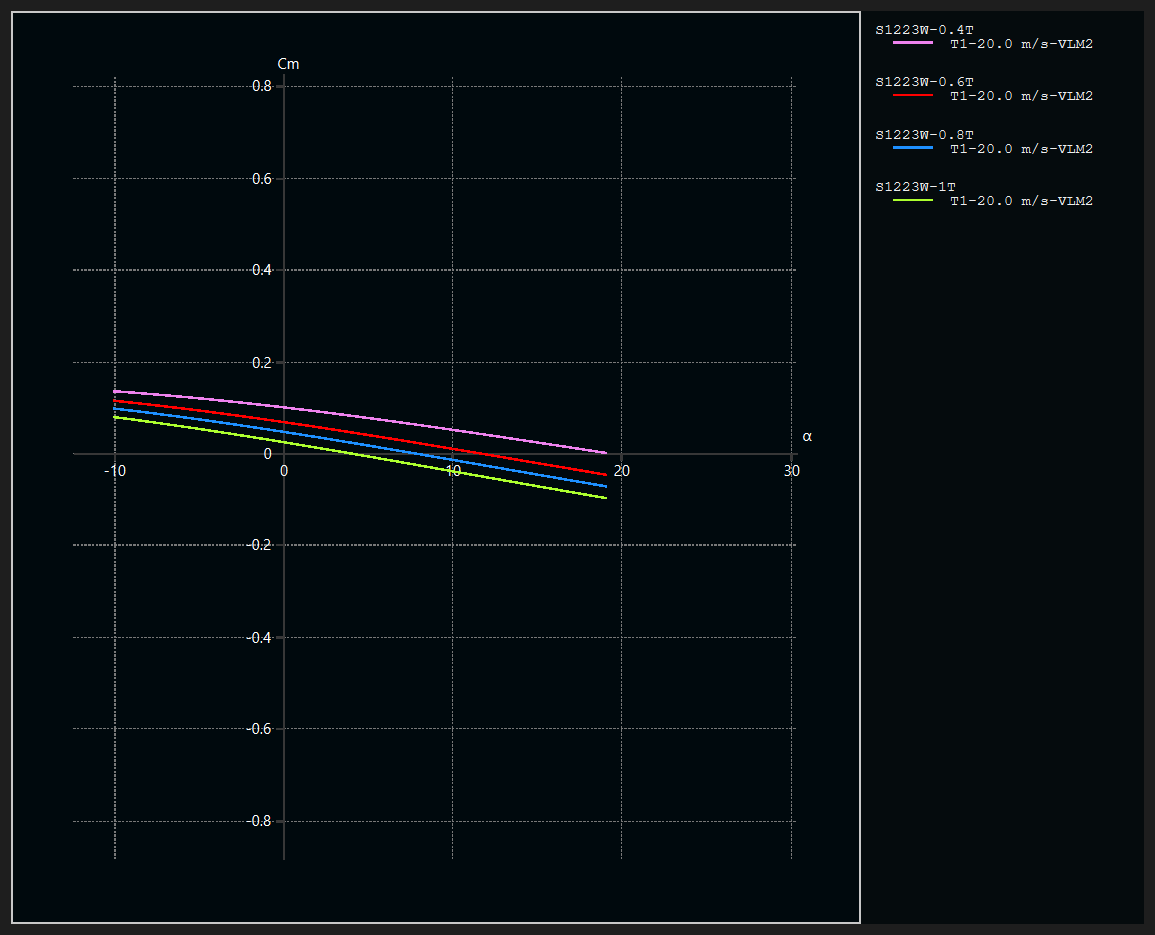
\includegraphics[width=0.9\textwidth]{Cm-alpha graph for HT.png}
\caption{Cm-$\alpha$ graph for Horizontal Tail ($0.4$ ,$0.6T$, $0.8T$, $1.0T$)}
\label{fig:wing_graphs}
\end{figure}

Based on the trade study, the \textbf{$\lambda= 0.6$ Variant} achieved the highest weighted score (4.60), successfully balancing optimal trim angle, superior aerodynamic efficiency, and ideal root-to-tip mass distribution.



\end{document}